\section{System Design}\label{sec:system}
LungAI has three parts (Fig.~\ref{fig:system}): a data pipeline that builds the training, validation and
test partitions (Section~\ref{sec:data}), a classifier and its training procedure
(Section~\ref{sec:method}), and a web application that serves the trained model.

\emph{Request path.} A user uploads a radiograph in the React frontend, which sends it to a FastAPI
backend. The backend first applies an input check that rejects images unlikely to be chest radiographs.
An accepted image passes through the same preprocessing code that was used in training and evaluation
and then through the classifier. The response contains the six class scores, the predicted class and a
Grad-CAM overlay \cite{selvaraju2017gradcam} computed on the last convolutional block. The prediction is
stored in an SQLite database with the model version and checkpoint hash, and the frontend offers a
history view, patient records, a plain-text report and a page with the evaluation metrics of the loaded
model.

\emph{Safeguards.} Four design decisions keep the application from presenting more than the model
supports. (i) The checkpoint is loaded only if its SHA-256 hash matches the value in the configuration.
(ii) If no verified model is loaded the prediction endpoint returns an error; there is no placeholder
output. (iii) A prediction whose highest score is below 0.5 is returned as inconclusive. (iv) Every
response carries a research-use notice and the external-evaluation limitation of
Section~\ref{sec:results}. The input check is heuristic: it was calibrated on validation radiographs and
has not been validated against a real set of non-radiograph images.

\emph{Implementation and testing.} The classifier is implemented in TensorFlow and all experiments run
on a laptop CPU. Automated tests cover the preprocessing, the metrics, the data-build scripts, the API
and the frontend services.

\begin{figure}[t]
\centering
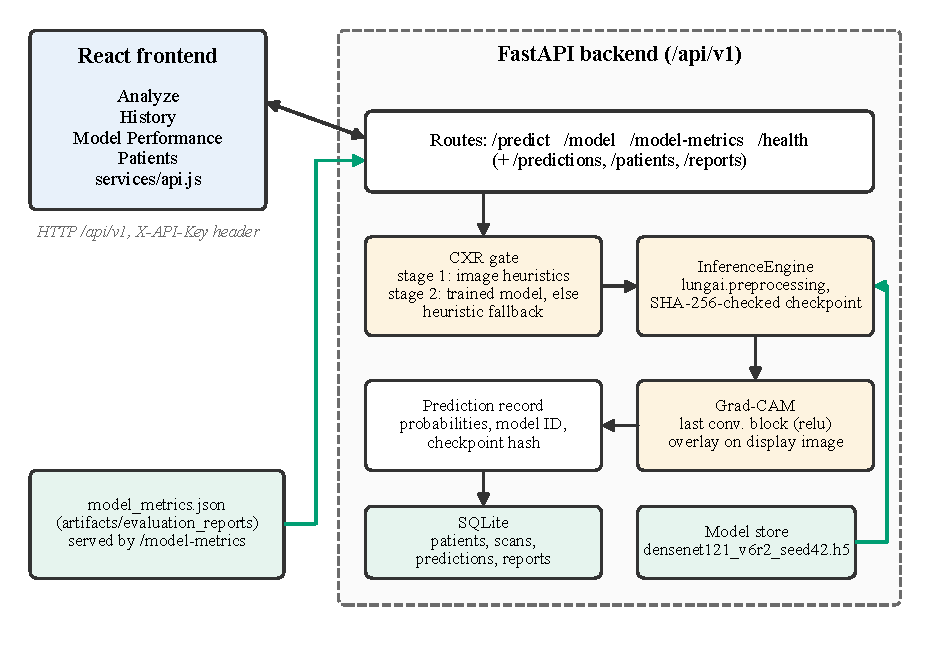
\includegraphics[width=\columnwidth]{../../figures/fig_system_architecture.pdf}
\caption{Architecture of the LungAI application: frontend, backend request path and stores.}
\label{fig:system}
\end{figure}
